\documentclass[12pt,oneside]{book}
\usepackage{amsmath,amssymb,amsthm,graphicx,enumitem,float,wrapfig}
\usepackage{fullpage}
\usepackage[utf8]{inputenc}
\usepackage[english]{babel}
\usepackage{perpage} %the perpage package
\MakePerPage{footnote} %the perpage package command
\usepackage{geometry}
\usepackage{marginnote}
\usepackage{lipsum}
\usepackage[inline]{asymptote}
\usepackage{subcaption}
\usepackage{cutwin}
\usepackage{microtype}
\graphicspath{ {./img/} }
\everymath{\displaystyle}

\catcode`\=13
\def{$\bowtie$}

\newcommand{\R}{\mathbb{R}}
\newcommand{\N}{\mathbb{N}}
\newcommand{\Z}{\mathbb{Z}}
\newcommand{\Q}{\mathbb{Q}}
\newcommand{\nhd}{neighborhood\space}
\newcommand{\ifnd}{if and only if\space}
\newcommand{\sq}{sequence\space}
\newcommand{\abs}[1]{\left\vert#1\right\vert}
\newcommand{\set}[1]{\left\{#1\right\}}
\newcommand{\seq}[1]{\left<#1\right>}
\newcommand{\sumnf}{\sum_{n=1}^{\infty}}

\theoremstyle{remark}
\newtheorem* {rem}{Remark}


\newtheorem{thm}{Theorem}[section]
\newtheorem{cor}[thm]{Corollary}
\theoremstyle{definition}
\newtheorem{prob}{Problem}[section]
\newtheorem{defn}{Definition}[section]
\newtheorem{ex}{Example}[section]
\newtheorem*{soln}{Solution}
\begin{document}
\title{Real Analysis}
\author{Mehedi Hasan}
\maketitle
\newpage
\pagenumbering{roman}
\tableofcontents
\newpage
\pagenumbering{arabic}
\chapter{Sets}
\section{Sets}
\begin{defn}[Supremum]
  Let $S\subset\R$. A number $u\in\R$ is said to an upper bound of $S$, if $s\leq u$ for all $s\in S$. If $S$ is bounded above, then the upper bound is said to be a supremum or a least upper bound (l.u.b) of $S$, written as sup $S=u$, if no number less than $u$ is an upper bound of $S$.
\end{defn}
\begin{defn}[Infimum]
  Let $S\subset\R$. A number $l\in\R$ is said to an lower bound of $S$, if $l\leq s$ for all $s\in S$. If $S$ is bounded below, then the lower bound $l$ is said to be a infimum or a greatest lower bound (g.l.b) of $S$, written as inf $S=l$, if no number greater than $l$ is an lower bound of $S$.
\end{defn}
\begin{figure}[h]
  \centering
  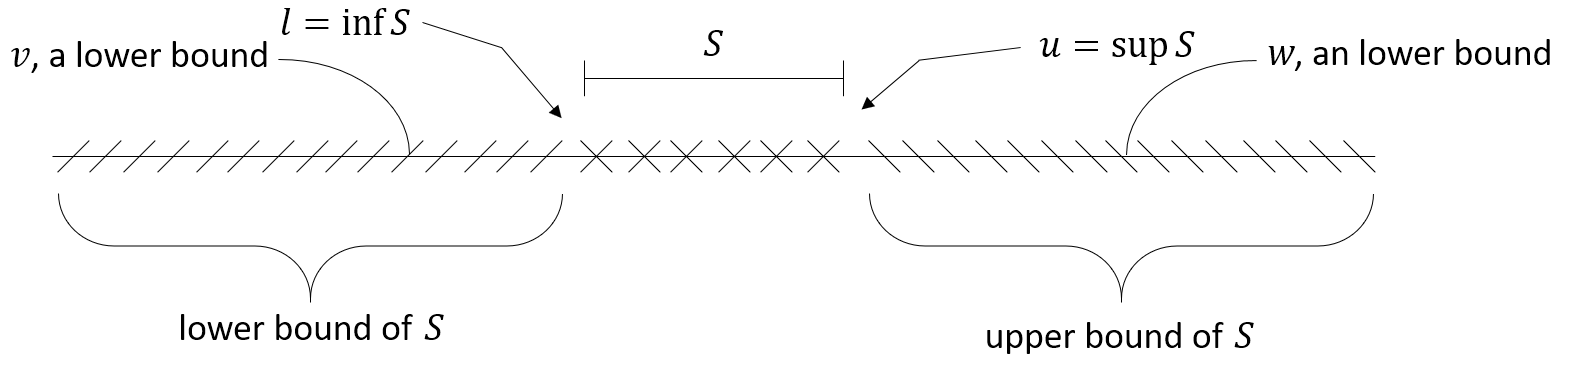
\includegraphics[scale=.5]{2}
  %\caption{}\label{}
\end{figure}
\begin{ex}
  $S=(0,1)\subset\R$, here $-1$ is a lower bound of $S$ and $2$ is an upper bound of $S$. clearly, sup $S=1$ and inf $S=0$.
\end{ex}
\begin{ex}
  $S=\left[\left.0,\infty\right)\right.$ inf $S=0$  and sup $S=\infty$ i.e., sup $S$ does not exist.
\end{ex}
\begin{ex}
  $S=\left(\left.-\infty,2\right.\right]$ inf $S=\infty$  i.e., inf $S$ does not exist and sup $S=2$
\end{ex}
\begin{ex}
  $S=\left\{\frac{1}{n}:n\in\N\right\}=\left\{1,\frac{1}{2},\frac{1}{3},\dots\right\}$ inf $ S=0$, sup $S=1$.
\end{ex}
\begin{thm}
  A number $u$ is a supremum of a nonempty subset $S$ of $\R$ \ifnd $ u$ satisfies the two conditions:
  \begin{enumerate}
    \item $s\leq u$ for all $s\in S$
    \item if $v<u$, then there exists an $s'\in S$ such that $v<s'$
  \end{enumerate}
\end{thm}
\textbf{Supremum Characterization}
\begin{thm}
  An upper bound $u$ of a non-empty set $S$ in $\R$ is the supremum of $S$ \ifnd for each $\varepsilon>0$, there exists an $s_\varepsilon \in S$ such that $u-\varepsilon<s_\varepsilon$
\end{thm}
\begin{proof}
  Suppose that $u$ is an upper bound of $S$ and satisfies the stated condition. If $v<u$ and we take $\varepsilon := u-v$, then $\varepsilon>0$, and the stated condition implies there exits a number $s_\varepsilon \in S$ such that $u-\varepsilon<s_\varepsilon$ i.e. $v<s_\varepsilon$ which implies that $v$ is not an upper bound of $S$. Since $v$ is an arbitrary number less than $u$, we conclude that $u=$sup $S$.\\

  Conversely, suppose that   $u=$sup $S$ and let $\varepsilon>0$. Since $u-\varepsilon<u$, then $u-\varepsilon$ is not an upper bound of $S$. Therefore, some elements $s_\varepsilon$ of $S$ must be greater than $u-\varepsilon$; that is, $u-\varepsilon<s_\varepsilon$
\end{proof}
\begin{figure}[h]
  \centering
  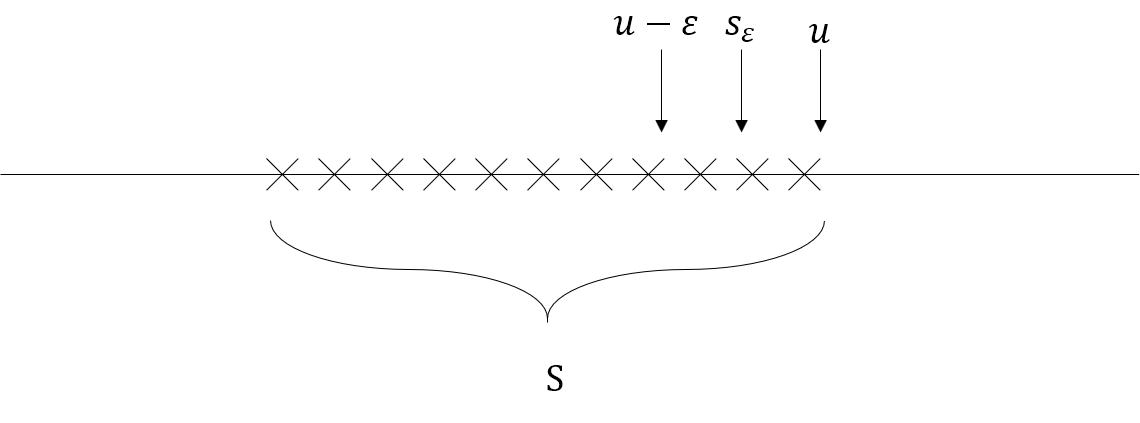
\includegraphics[scale=.5]{3}
  %\caption{}\label{}
\end{figure}
\fbox{Obtain the \emph{infimum characterization.}}
\begin{ex}
  Let $S=(a,b), a,b \in \R$. Show that sup $S=b$ and inf $S=a$.
\end{ex}
\begin{soln}
  Observe that $b$ is an upper bound of $S$ because $s\leq b$ for all $s\in S$. Now given $\varepsilon>0,\,b-\varepsilon<b$. Clearly $b-\varepsilon \in S$, so there exits an $s_\varepsilon\in S$ such that $b-\varepsilon<s_\varepsilon$.\\
  Hence by supremum characterization we have $b=$sup $S$.\\
  Similarly, by using infimum characterization $a=$inf $S$.
\end{soln}
\begin{defn}[Maximum of a Set]
  Let $S\subset\R$. Then an element $m\in S$ is called the maximum(or the greatest or the largest) element of $S$ if $s\leq m$ for all $s\in S$.
\end{defn}
\begin{defn}[Minimum of a Set]
  Let $S\subset\R$. Then an element $l\in S$ is called the minimum(or the least or the smallest) element of $S$ if $l\leq s$ for all $s\in S$.
\end{defn}
\begin{ex}
  $S=\left.\left[1,2\right.\right)$. min $S=1$, max $S$ does not exist.
\end{ex}
\begin{ex}
  The sets $\Z$ and $\Q$ have neither maximum nor minimum. The set $\N$ has no maximum but has a minimum. i.e. min $\N=1$.
\end{ex}
\emph{Triangle Inequality} $\big||x|-|y|\big|\leq|x-y|\leq|x+y|\leq|x|+|y|$
\subsection{The Completeness Property of the set of Real Number $\R$}
Here we shall present a special property of $\R$ that is often called the "Completeness property", since it guarantees the \emph{existence of elements in $\R$} under certain hypothesis. We know that $\sqrt{2}$ is not a rational number, i.e. $\sqrt{2}\notin \Q$. This observation shows the necessity of an additional property to characterize the real number system. This additional property, the Completeness property, is an essential feature of $\R$.\\

There are several different versions of the Completeness property. Such as,
\begin{enumerate}[label=(\roman*)]
  \item The supremum Property (or The Infimum Property)
  \item Dedikind's Axiom.
  \item Cauchy Completeness Property.
\end{enumerate}
\textbf{The supremum property of the real number system $\R$:}\\
Every non empty set of real numbers that has an upper bound has a supremum is $\R$.\\

The analogues infimum property of the real number system $\R$ states that, "Every non empty set of real numbers that has a lower bound has an infimum in $\R$."\\

One important consequence of the supremum property is that the subset $\N$ of natural numbers is not bounded above in $\R$. This means that given any real number $x$ there exists a natural number $n$ (depending on $x$) such that $x<n$.\\

\textbf{Archimedean Property:} If $x\in\R$, then there exists $n_x\in \N$ such that $x<n_x$.
\begin{proof}
  If the conclusion fails, then $x$ is an upper bound of $\N$. Therefore by the supremum property, the non empty set $\N$ has a supremum $u\in\R$. Since $u-1<u$, it follows from the previous supremum characterization theorem that there exists $m\in\N$ such that $u-1<m$. But then $u<m+1$ and since $m+\in\N$, this contradicts the assumption that $u$ is an upper bound of $\N$.
\end{proof}
\begin{cor}
  Let $y$ and $z$ be positive real numbers. Then\\
  \begin{enumerate}[label=(\roman*)]
    \item There exists $n\in\N$ such that $z<ny$
    \item There exists $n\in\N$ such that $o<\frac{1}{n}<y$
    \item There exists $n\in\N$ such that $n-1\leq z<n$
  \end{enumerate}
\end{cor}
\textbf{Homework:} Let $S$ be a non empty subset of $\R$ that is bounded above and let $a\in\R$. Define the set $a+s=\set{a+x:x\in S}$. Show that sup $(a+S)=a+$ sup $S$.
\subsection{Open and Closed Sets in $\R$}
\begin{defn}[Neighborhood]
  Let $a\in \R$ and $\varepsilon >0$. Then the $\varepsilon$-neighborhood of $a$ is the set $N_\varepsilon=\{x\in\R:|x-a|<\varepsilon\}$.
\[|x-a|<\varepsilon\quad\Rightarrow\,a-\varepsilon<x<a+\varepsilon\]
\begin{figure}[h]
  \centering
  
\includegraphics{1}
  \caption{A $\varepsilon-$neighborhood of $a$}\label{fig:epsilonNhd}
\end{figure}

\end{defn}
\begin{defn}[Open Set]
  Let $S\subset\R $ and $x\in S$, then $S$ is an open set if $N_\varepsilon(x)\subset S$. Generally, open set is denoted by $G$.
\end{defn}
\subsection{Properties of Open Set}
\begin{enumerate}[label=(\alph*)]
  \item The union of an arbitrary collection of open sets in $\R$ is open.
  \item The intersection of any finite collection of open sets on $ \R$ is open.
\end{enumerate}
\begin{proof}
  \begin{enumerate}[label=(\alph*)]
    \item Let $\{G_\lambda:\lambda\in\Lambda\}$ be a family of sets in $\R$ that are open, and let $G$ be their union; by the definition of union, $x$ must belong to $G_{\lambda_0}$ for some $\lambda_0\in\Lambda$. Since $G_{\lambda_0}$ is open, there exists a \nhd $V$ of $x$ such that $V\subseteq G$. But $G_{\lambda_0}\subseteq G$, so that $V\subseteq G$. Since $ x$ is an arbitrary element of $G$, we conclude that $G$ is open in $\R$.\\

        \footnote{This is from class}$\{G_\lambda:\lambda\in\Lambda\}$ is an arbitrary collection of open set.
        \[G=\cup G_\lambda\quad x\in G\Rightarrow N_\varepsilon (x)\subset G\]
        \begin{align*}
           & x\in G \\
          \Rightarrow\, & x\in \cup G_\lambda \\
          \Rightarrow\, & x\in \cup G_{\lambda_0}\quad\quad \lambda_0\in\Lambda \\
          \Rightarrow\, & N_\varepsilon (x)\subset G_{\lambda_0}\subset G
        \end{align*}
        $G$ is open if $x\in G\Rightarrow N_\varepsilon (x)\subset G$
    \item Suppose $G_1$ and $G_2$ are open and let $G := G_1\cap G_2$. To show that $G$ is open, we consider any $x\in G$; then $x\in G_1$ and $x\in G_2$. Since $G_1$ is open, there exits $\varepsilon_1>0$ such that $(x-\varepsilon_1,x+\varepsilon_1)$ is contained in $G_1$. Simillarly, since $G_2$ is open, there exits $\varepsilon_2>0$ such that $(x-\varepsilon_2,x+\varepsilon_2)$ is contained in $G_2$. If we now take $\varepsilon$ to be smaller of $\varepsilon_1$ and $\varepsilon_2$, then the $\varepsilon-$\nhd $U:=(x-\varepsilon,x+\varepsilon)$ satisfies both $U\subseteq G_1$ and $U\subseteq G_2$. Thus, $x\in U\subseteq G$. Since $x$ is an arbitrary element of $G$, we conclude that $G$ is open in $\R$.\\

        \footnote{This is from class}
        \begin{align*}
          G & =\cap_{\lambda=1}^N G_\lambda \\
           & =G_1\cap G_2\cap G_2\cap \dots \cap G_n \\
           G & =G_1\cap G_2
        \end{align*}
        \begin{align*}
           & x\in G \\
          \Rightarrow\, & x\in G_1\quad \text{and}\quad  x\in G_2\\
          \Rightarrow\, & N_{\varepsilon_1}(x)\subset G_1\quad \text{and}\quad  N_{\varepsilon_2}(x)\subset G_2
        \end{align*}
        $\varepsilon=\text{min}\{\varepsilon_1,\varepsilon_2\}$
        \begin{align*}
           & N_{\varepsilon}(x)\subset G_1\quad \text{and}\quad  N_{\varepsilon}(x)\subset G_2 \\
          \Rightarrow\, & N_{\varepsilon_1}(x)\subset G_1\cap G_2=G
        \end{align*}
  \end{enumerate}
\end{proof}
\begin{defn}[Closed Set]
  A set $F\subset\R$ is called closed set if $F^c$ is open set. Generally, close set is denoted by $F$.
\end{defn}
\subsection{Properties of Closed Set}


\begin{enumerate}[label=(\alph*)]
  \item The intersection of an arbitrary collection of closed sets in $\R$ is closed.
  \item The union of any finite collection of closed sets in $\R$ is closed.
\end{enumerate}
\begin{proof}
  \begin{enumerate}[label=(\alph*)]
    \item If $\{F_\lambda :\lambda\in\Lambda\}$ is a family of closed sets in $\R$ and $F:=\cap_{\lambda\in\Lambda} F_\lambda$, then $C(F)=\cup_{\lambda\in \Lambda}$ is the union of open sets. Hence, $C(F)$ is open by properties of open set(a) and consequently, $F$ is closed.
    \item Suppose $F_1,F_2,\dots,F_n$ are closed in $\R$ and let $F:=F_1\cup F_2\cup\dots\cup F_n$. By the De Morgan identity of the complement\footnote{$(A\cup B)^c=A^c\cap B^c$ and $(A\cap B)^c=A^c\cup B^c$} of $F$ is given by
        \[C(F)=C(F_1)\cap\dots\cap C(F_n)\]
        Since each set $C(F_i)$ is open, it follows properties of open set(b) that $C(F)$ is open. Hence $F$ is closed.
  \end{enumerate}
\end{proof}
\chapter{Series and Series of Function}
\section{Sequence}
\begin{defn}[Sequence]
  A sequence of real numbers (or a sequence in $\R$)is a function defined on the set $\N = {1, 2,\dots}$ of natural numbers whose range is contained in the set $\R$ of real
numbers.
\end{defn}
Since $\N$ is the domain of a sequence $x(n)=x_n$ so a sequence is an ordered set and is denoted by $\seq{x_n}$ or $(x_n)$.
\begin{rem}
A \sq is a set of real numbers with an order.
\end{rem}
\begin{ex}
\begin{enumerate}
  \item   $\seq{x_n}=\seq{\frac{1}{n}}=\seq{1,1/2,1/3,\dots,1/n,\dots}$
  \item $\seq{x_n}=\seq{n}$
  \item $\seq{x_n}=\seq{(-1)^n}$
\end{enumerate}
\end{ex}
\section{Series}
\begin{defn}[Series]
  Sum of the terms of an infinite sequence is called series. Given a series $\sum_{n=1}^{\infty}x_n=x_1+x_2+x_3+\dots,$ let $s_n$ denote its $n-$th partial sum:
  \[
  s_n=\sum_{k=1}^{n}x_k =x_1+x_2+x_3+\dots+x_n.
  \]
  If the sequence $s_n$ is convergent, i.e. if $x$ is a real number such that $\lim(s_n)=x$, then the series $\sum x_n$ is called \emph{convergent} and we write
  \[
  \lim_{n\rightarrow\infty}\sum_{k=1}^{n}x_k =\sum_{k=1}^{\infty}x_k= x_1+x_2+x_3+\dots=x
  \]
  The number $x$ is called the sum of the series. Otherwise, the series is \emph{divergent}.\\
  Note that $\sum_{k=1}^{\infty}x_k=\lim_{n\rightarrow\infty}\sum_{k=1}^{n}x_k$
\end{defn}
\begin{thm}
  The geometric series
  \[
  \sum_{n=1}^{\infty}ar^{n-1}=a+ar+ar^2+\dots
  \]
  is convergent if $\abs{r}<1$ and its sum is
  \[
  \sum_{n=1}^{\infty}ar^{n-1}=\frac{a   }{1-r}\qquad\abs{r}<1
  \]
  if $\abs{r}\geq 1$, the series is divergent.
\end{thm}
\begin{ex}
  Test whether the series $\sum_{n=1}^{\infty}2^{2n}3^{1-n}$ is convergent or divergent.
\end{ex}
\begin{soln}
  $\sum_{n=1}^{\infty}2^{2n}3^{1-n}=\sum_{n=1}^{\infty}4(4/3)^{n-1}$ is a geometric series with $a=4$ and $r=4/3\,>1$. So, the series is divergent.
\end{soln}
\begin{thm}
  The $p-$ series $\sumnf \frac{1}{n^p}$ is convergent if $p>1$ and divergent if $p\leq 1$. When $p=1$ the series is called  the \emph{harmonic} series.
\end{thm}
\begin{thm}
  If the series $\sumnf x_n$ is convergent, them $\lim(x_n)=0$. But the converse is not true in general, e.g, harmonic series.
\end{thm}
\begin{thm}[The Test for Divergent]
  If $x_n \rightarrow \infty$ or $x_n \nrightarrow 0$ then the series $\sumnf x_n$ is divergent.
\end{thm}
\begin{ex}
  Test whether the series $\sumnf \frac{n^2}{5n^2+4}$ is convergent or divergent.
\end{ex}
\begin{soln}
  Here $x_n=\frac{n^2}{5n^2+4}\rightarrow1/5\neq0$ so the test for divergence implies that the series is divergent.
\end{soln}
\begin{thm}
  The sum, difference, and scalar multiple of two convergent series are convergent.
\end{thm}
\begin{ex}
  Find the sum of the series $\sumnf \left( \frac{3}{n(n+1)}+\frac{1}{2^n}\right)$
\end{ex}
\begin{soln}
  Here the second series is geometric series with $a=1/2$ and $r=1/2$, so $\sumnf \frac{1}{2^n}=\frac{a}{1-r}=1$. The first series is $\sumnf \frac{3}{n(n+1)}=3\lim_{n\rightarrow\infty}\sum_{i=1}^{n}\frac{1}{i(i+1)}=\lim_{n\rightarrow\infty}(1-\frac{1}{n+1})=3$. Therefore the sum of the given series is $3+1=4$.
\end{soln}
\begin{thm}[Cauchy Criterion for Series b]
  A series $\sum x_n$ in $\R$ is convergent iff for each $\epsilon>0$ there is a natural number $K:=K(\epsilon)$ such that if $m>n\geq K$, then
  \[
  \abs{s_m-s_n}=\abs{x_{n+1}+x_{n+2}+\dots+x_m}<\epsilon
  \]
\end{thm}
\begin{defn}
  We say that a series $\sum x_n$ is absolutely convergent if the series $\sum\abs{x_n}$ is convergent in $\R$. A series is conditionally convergent if it is convergent but not absolutely convergent.
\end{defn}
\begin{thm}
  If a series is absolutely convergent, then it is convergent.
\end{thm}
\subsection{Tests for Absolute Convergence}
\begin{thm}[Comparison Test b]
  Let $x_n$ and $y_n$ be real sequences such that for some natural number $K$,
  \[
  0\leq x_n\leq y_n\qquad\text{for } x\geq K
  \]
  Then the convergence of $\sum y_n$ implies the convergence of $\sum x_n$ and the divergence of $\sum x_n$ implies the divergence of $\sum y_n$.
\end{thm}
\begin{ex}
  Test the convergence of the series $\sumnf \frac{5}{2n^2+4n+3}$
\end{ex}
\begin{soln}
  Note that $\frac{5}{2n^2+4n+3}<\frac{5}{2n^2}$ by the $p-$ series $\sum \frac{1}{n^2}$ converges and hence by the comparison test the given series is convergent.
\end{soln}
\begin{thm}[Limit Comparison Test b]
  Let $x_n$ and $y_n$ be positive real sequences and $L=\lim(x_n/y_n)$
  \begin{enumerate}
    \item If $L\neq 0$, then $\sum x_n$ is convergent iff $\sum y_n$ is convergent.
    \item If $L=0$ and $\sum y_n$ is convergent then $\sum x_n$ is convergent.
  \end{enumerate}
\end{thm}
\begin{ex}
  Test the convergence of the series $\sumnf \frac{2n^2+3n}{\sqrt{5+n^5}}$.
\end{ex}
\begin{soln}
  Note that the dominant part od the numerator is $2n^2$ and the dominant part of the denominator is $\sqrt{n^5}$. This suggests taking $x_n=\frac{2n^2+3n}{\sqrt{5+n^5}},$ $y_n=\frac{2n^2}{\sqrt{n^5}=\frac{2}{n^{1/2}}}$ $\lim_{n\rightarrow\infty}\frac{x_n}{y_n}=\lim_{n\rightarrow\infty}\frac{2n^2+3n}{\sqrt{5+n^5}}\times\frac{n^{1/2}}{2}=1$ Since $\sum y_n=2\sum 1/n^{1/2}$ is divergent (p-series with $ p=1/2<1$)
\end{soln}
\begin{thm}[Root test b]
  Let $x_n$ be a sequence in $\R$ and \[
  r:=\lim(\abs{x_n}^{1/n}).
  \]
  Then $\sum x_n$ is absolutely convergent if $r<1$ and divergent if $r>1$.
\end{thm}
\begin{ex}
  Test the series $\sumnf \left(\frac{2n+3}{3n+2}\right)^n$
\end{ex}
\begin{soln}
  Root test with $x_n=\left(\frac{2n+3}{3n+2}\right)^n$ gives $ \sqrt[n]{\abs{x_n}}=\frac{2n+3}{3n+2}\rightarrow2/3<1$. Thus, the given series is convergent by the root test.
\end{soln}
\begin{thm}[Ratio test b]
  Let $x_n$ be a sequence in $\R$ and
  \[
  r:=\lim(\abs{x_{n+1}}/\abs{x_n})
  \]
  Then $\sum x_n$ is absolutely convergent if $r<1$ and divergent if $r>1$
\end{thm}
\begin{ex}
  Test the series $\sumnf (-1)^n\frac{n^3}{3^n}$ for absolute convergence.
\end{ex}
\begin{soln}
  Ratio test with $x_n=(-1)^n\frac{n^3}{3^n}$ gives: $\abs{\frac{a_{n+1}}{a_n}}=\abs{\frac{1}{3}\frac{n+1}{n}^3}=\abs{\frac{1}{3}(1+1/n)^3}\rightarrow\frac{1}{3}<1$.
  Thus, by ratio test, the given series is absolutely convergent and therefore convergent.
\end{soln}
\begin{thm}[Raabe's Test b]
  Let $x_n$ be a sequence of nonzero real numbers and
  \[r:=\lim(n(1-\frac{\abs{x_{n+1}}}{\abs{x_n}})
  \]
  Then $\sum x_n$ is absolutely convergent if $r>1$ and is not absolutely convergent if $r<1$.
\end{thm}
\begin{thm}[Integral Test b]
  Let $f$ be a continuous, positive decreasing function on $\left.\left[1,\infty\right.\right)$ and $x_n=f(n)$. Then if $ \int_{1}^{\infty}f(x)\mathrm{d}x$ is convergent (divergent), then $\sum x_n$ is convergent (divergent).
\end{thm}
\begin{ex}
  Test the series $\sumnf \frac{\ln n}{n}$ for convergence.
\end{ex}
\begin{soln}
  The function $f(x)=\frac{\ln x}{x}$ is positive and continuous for $x>1$ because the logarithm function is continuous. But it is not clear whether or not $f$ is decreasing, so $f'(x)=\frac{1-\ln x}{x^2}$ Thus, $f'(x)<0$ when $1-\ln x<0$ i.e., $x>e$. So $f$ is decreasing when $x>e$. Here $\int_{1}^{\infty}\frac{\ln x}{x}\mathrm{d}x=\lim_{t\rightarrow\infty}\int_{1}^{t}\frac{\ln x}{x}\mathrm{d}x=\infty$. Therefore, by the integral test the given series is divergent.
\end{soln}
\subsection{Test For Nonabsolute Convergence}
\begin{defn}[Alternating Series]
  An alternating series is a series whose terms are alternately positive and negative. The $n-$th term of an alternating series is defined by $x_n=(-1)^{n-1} y_n$, $x_n=(-1)^{n} y_n$,$x_n=(-1)^{n+1} y_n$ where $n\in\N$ and $y_n>0$
\end{defn}
\begin{thm}[Alternating Series Test b]
  Let $x_n$ be a decreasing sequence of positive real numbers with $\lim(x_n)=0$. Then the alternating series $\sum (-1)^{n+1} x_n$ is convergent.
\end{thm}
\begin{ex}
  Test the convergence of the series $\sumnf\frac{(-1)^{n+1}}{n}$, $\sumnf\frac{(-1)^{n+1}}{\sqrt{n}}$
\end{ex}
\end{document} 